% Created 2014-05-11 Sun 15:34
\documentclass[a4paper,6pt]{article}
\usepackage[utf8]{inputenc}
\usepackage[T1]{fontenc}
\usepackage{fixltx2e}
\usepackage{graphicx}
\usepackage{longtable}
\usepackage{float}
\usepackage{wrapfig}
\usepackage{rotating}
\usepackage[normalem]{ulem}
\usepackage{amsmath}
\usepackage{textcomp}
\usepackage{marvosym}
\usepackage{wasysym}
\usepackage{amssymb}
\usepackage{hyperref}
\tolerance=1000
\usepackage[margin=.75in]{geometry}
\usepackage[T1]{fontenc}
\usepackage[scaled=.7]{helvet}
\usepackage{courier} % tt
\linespread{1.01}
\author{N-CRITSER}
\date{\textit{<2014-05-06 Tue>}}
\title{267\_writeup.org}
\hypersetup{
  pdfkeywords={},
  pdfsubject={},
  pdfcreator={Emacs 23.4.1 (Org mode 8.2.4)}}
\begin{document}

\maketitle



\section{Abstract "TALK-A-LOT-BOT" v.0}
\label{sec-1}
    My original goal for this project was to learn the underlying code for 
the Arduino platform while creating an anthropomorphic entity which "speaks"
and simulates eye movement while interacting with a user.  The general aspects
of this I have achieved, although I have adopted the usage of higher level 
libraries and forgone the learning of lower level aspects of the platform.  

    Currently the Talk-a-lot-Bot has as its central processing unit a Rev3 
Arduino Uno with an Ada-fruit Waveshield mounted to its I/O headers. The shield
controls the robots "voice" and plays pre-recorded .WAV files, through a 
3.5 mm stereo (TRS) plug that feeds the sound to and 8 ohm speaker.  The .WAV files  are stored on a 
Fat 16 Formatted SD card.  The arduino sketch code processes the .WAV files and makes them 
playable by name.  We use the file names and flag value settings in the code to determine 
which file should be played.  


    Also, connected to the Uno, are 2 8x8 LED matrices, which are I2C protocol driven. This means
we can save a lot of I/O pins and still get a lot of variability in our eye movement.  The I2C backPacks
for the matrices use only Power,Ground,  and 2 analog pins from the UNO (A4, A5), for clock and data.  Each 
matrix has an address that is set in code as well as selected on the matrix backPack itself by making a 
solder bridge between open pads on the small backPack pcb.  This addressing is explicitly controlled in 
the sketch code which makes the backPacks independent.  

    Housing the components are two sheets of ABS plastic.  This material is a great substrate 
for electronics as well as oil paint and has a lot of fantastic properties.  It's very maliable,
easy to cut, and can dissipate heat fairly well.  I have cut holes for the eye matrices and 
attached the UNO and other components via bolts.  For the first iteration I have kept the button pad
as a seperate unit attached only by plugged (not soldered wires).  

    On the button front, we have 3 simple push buttons, each with an LED that is set high while the button
is HIGH and LOW when the button is pressed.  This scheme helps the user know how long a button has been 
pressed, while also giving a visual debug of the button pin itself.  The interaction between the Digital
I/O pins have been a slight mystery.  The UNO pins 11,12,13 are not technically used for the wave shield
but if buttons are connect to pins, they act as an interrupt on the .WAV playing object.  While, Pins 0,1 are 
free from this side effect behavior.  This can be used as a way to cut short the Talk-A-lot-Bot if you feel 
he's talking too much.  But otherwise it is a nuisance.  And if an interrupt button is held down while the play 
flag for a .WAV file is being loaded, then the shield is unable to play the file and a few loop cycles are needed 
to reset the system.  

    Initially I wanted T.A.L.B. to play a Binary Search game with the user, but after struggling to adjust the 
buttons with the .WAV in a fun way, I decided to take some inspiration from an early soft bot known as PARRY. 
\url{http://en.wikipedia.org/wiki/PARRY}.  PARRY  was supposed to simulate a paranoid schyzophrenic and was one of the first 
bots to pass the Turing Test.  Currently, I think T.A.L.B. doens't quite pass the Turing Test, but maybe version 1 will. 
\section{Components}
\label{sec-2}
\subsection{Adafruit waveshield sd card module}
\label{sec-2-1}
\url{https://www.adafruit.com/products/94}

\subsection{Speaker}
\label{sec-2-2}
Description for lady Ada-
"Speaker - 3" diameter (77mm), 8 ohm impedence, good response 
between 200Hz to 10KHz (10KHz is the max frequency 
the Wave shield can make). The speaker is rated for 
1W so if you want you can even stick a small amp 
between the shield and the speaker to boost up the volume"

\subsection{Arduino Uno Rev3 Microcrontroller}
\label{sec-2-3}
\subsection{2-8x8 i2c led matrices for simulated eye movement}
\label{sec-2-4}
\url{https://www.adafruit.com/products/872}

\subsection{adafruit libraries for graphics and sound}
\label{sec-2-5}
\section{Libraries}
\label{sec-3}
\begin{verbatim}
#include "Adafruit_LEDBackpack.h"

#include "Adafruit_GFX.h"
\end{verbatim}

\section{Wiring Diagram}
\label{sec-4}
The Following diagram shows only the UNO and I2C Matrices, I have included the WaveShield Schematic from Lady Ada
in the following section. 

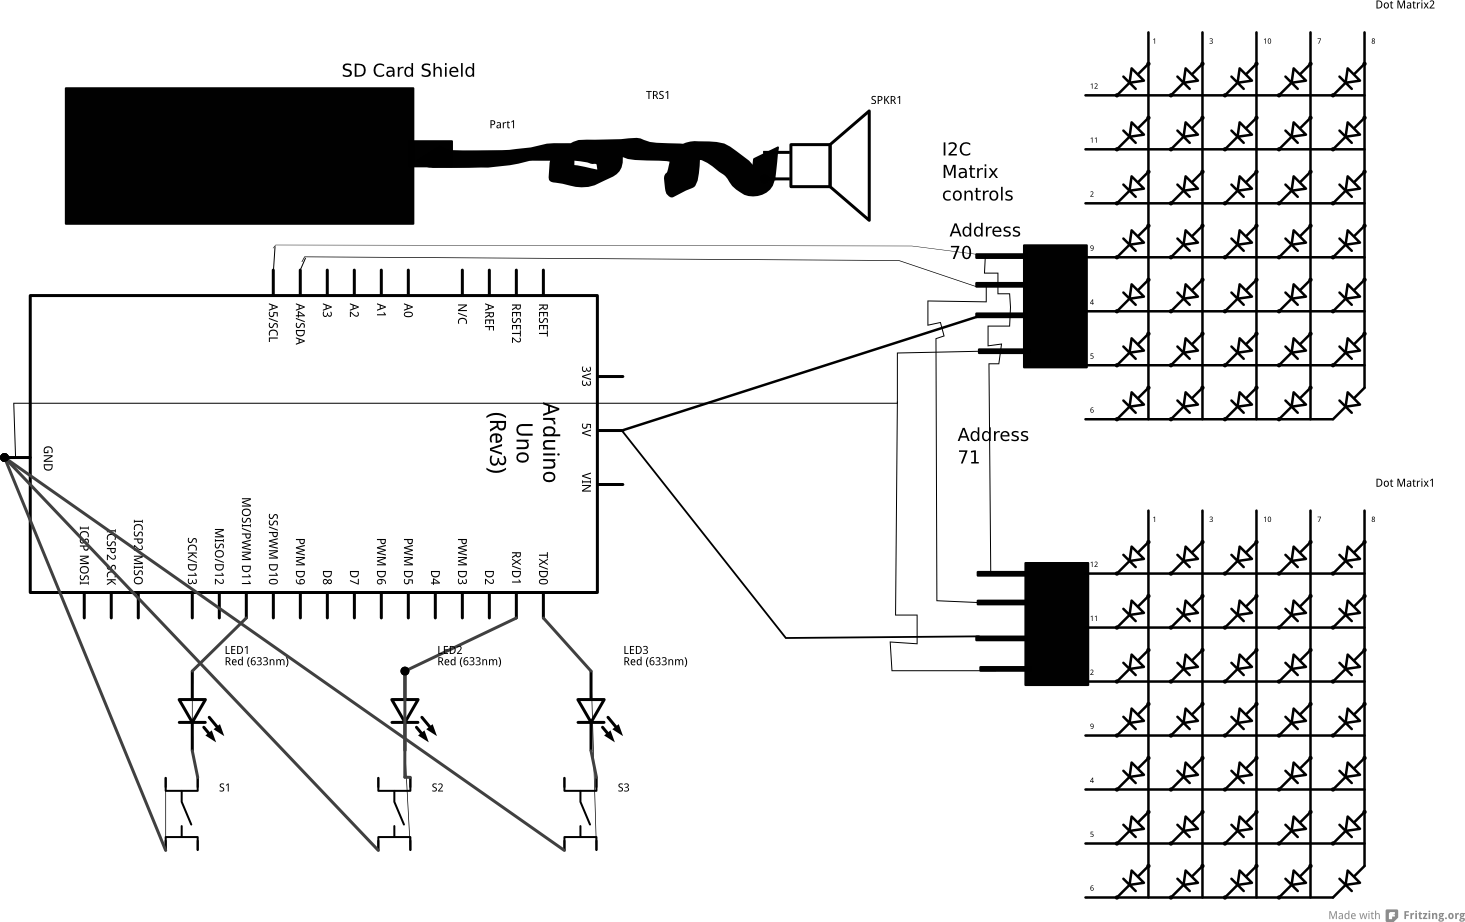
\includegraphics[angle=0,width=16cm]{./talk_a_lot_wire.png}
\section{WaveShield Diagram}
\label{sec-5}
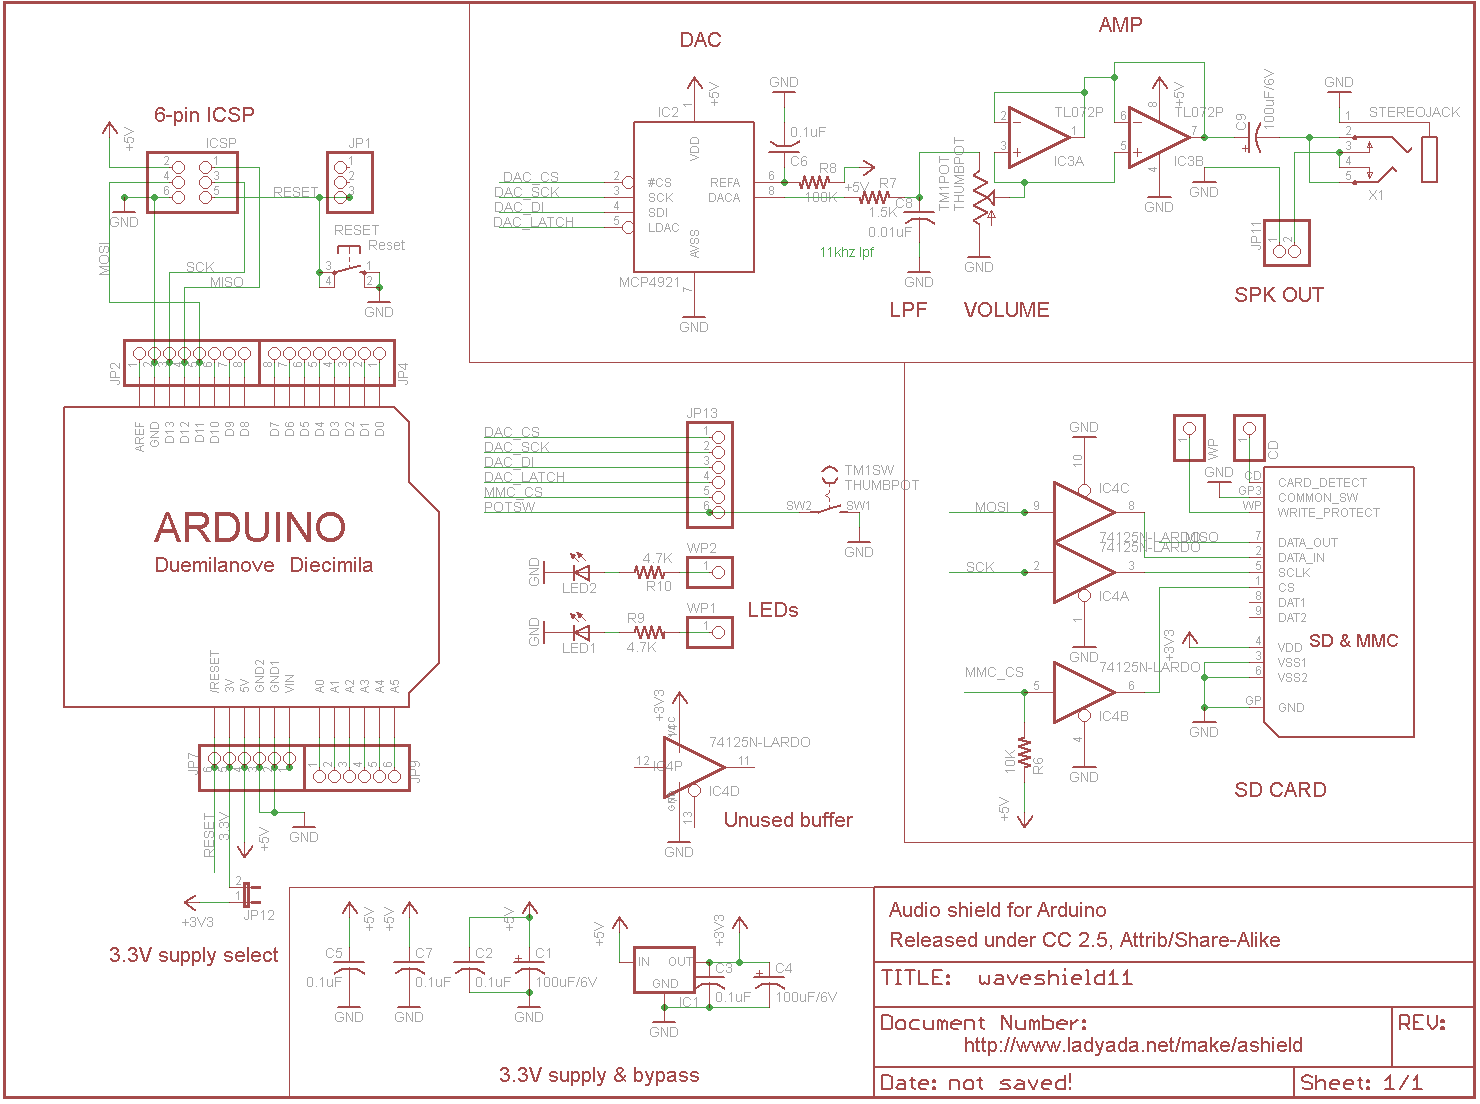
\includegraphics[angle=0,width=16cm]{./wave11schem.png}
% Emacs 23.4.1 (Org mode 8.2.4)
\end{document}
